% ch-parallel.tex -- shared-memory parallelism, what scales and what does not
\chapter{Running in parallel}
\label{ch:parallel}

Yuzen is parallelized with OpenMP. This chapter says what that gets you, what
it does not, how many threads to ask for, and --- because the honest answer
depends on the case --- what was actually measured.

\begin{warn}[There is no distributed-memory parallelism]
  \textbf{Yuzen has shared-memory parallelism only. It does not support MPI,
  and there is no MPI version planned.} One run is one process on one machine,
  using several threads inside it. Two consequences follow. The largest problem
  you can solve is bounded by the memory of a single node, and it cannot be
  made larger by adding nodes. And a cluster is useful to you only as a way of
  running \emph{several cases at once}, one process each --- which is in any
  case the more efficient use of it, since a single case scales far less well
  than a queue of independent cases.
\end{warn}

\section{Choosing the thread count}
\label{sec:parallel:threads}

The thread count comes from \env{OMP\_NUM\_THREADS} in the usual way; there is
no input key for it.

\begin{shell}
OMP_NUM_THREADS=2 ./build/bin/yuzen cases/leveling_2d_fine_reg.toml
\end{shell}

\begin{warn}[Never ask for more threads than you have physical cores]
  Over-subscription is not a small loss, it is a catastrophe. On a two-core
  Xeon at \SI{2.1}{\giga\hertz}, running four threads on
  \file{leveling\_1d\_reg} costs a factor of three to six against one thread; an
  in-house backend tried during development lost a factor of ten the same way ---
  \SI{93}{\second} against \SI{9.4}{\second} on one thread. Set
  \env{OMP\_NUM\_THREADS} to the physical core count or below, and do not rely
  on the default, which on a machine reporting hyper-threads will be too high.
\end{warn}

\begin{warn}[Cores that are busy count as missing]
  The same catastrophe follows when the cores exist but something else is
  using them: a second run, a build, \code{ctest -j}. The OpenMP runtime
  spins at the end of every parallel loop, and a step makes thousands of
  short ones; with a thread waiting for a core instead, every one of them
  costs a scheduler slice. On the two-core machine, with one core busy,
  \code{concz\_vs\_wm} took \SI{246}{\second} on two threads against
  \SI{5}{\second} with \env{OMP\_WAIT\_POLICY=passive}. If you share the
  machine, either leave the threads at one per free core or set
  \env{OMP\_WAIT\_POLICY=passive}; the answer is the same either way.
  \code{ctest} sets it for the tests that run the solver.

  \textbf{When the cores are yours, leave \env{OMP\_WAIT\_POLICY} unset.}
  \val{passive} puts a sleep and a wake-up into every one of those loops. On
  a Xeon Max 9480 node an empty parallel loop costs \SI{1.7}{\micro\second}
  on 8 threads and \SI{24}{\micro\second} on 112 with the policy unset, and
  \SI{25}{\micro\second} and \SI{258}{\micro\second} with \val{passive}
  (\file{tools/\bk scaling/\bk omp\_overhead.cpp}); on a dedicated node the
  setting that rescues a shared machine makes every multi-threaded run
  slower.
\end{warn}

\subsection{The OpenMP runtime}
\label{sec:parallel:runtime}

Every parallel loop costs a fork and a join whatever the work inside it, and a
step makes thousands of them. How much that costs depends on the OpenMP
\emph{runtime} the solver is linked to more than on anything in the solver.
On a socket of a Xeon Max 9480 (56 cores), an empty parallel loop costs:

\begin{yzntable}{The cost of one empty parallel loop, \si{\micro\second}, by runtime and thread count (\file{tools/\bk scaling/\bk omp\_overhead.cpp}, \env{OMP\_PROC\_BIND=close}).\label{tab:omp-runtime}}{@{}L{0.42\textwidth} d d d d@{}}
\textsf{\bfseries Runtime} & \textsf{\bfseries 8} & \textsf{\bfseries 16} & \textsf{\bfseries 28} & \textsf{\bfseries 56} \\ \midrule
  GCC's \code{libgomp}                      & 1.6 & 2.5 & 4.0 & 8.0 \\
  LLVM's \code{libomp}, with GCC's code      & 1.0 & 1.4 & 1.6 & 2.1 \\
  Intel's \code{libiomp5}, with \code{icpx}  & 1.0 & 1.4 & 1.7 & 2.1 \\
\end{yzntable}

\code{libgomp} grows about in proportion to the thread count;
the other two barely grow. \textbf{A GCC build therefore links LLVM's
\code{libomp} instead of \code{libgomp} when \code{libomp} is installed}
(the package \code{libomp-dev} on Debian and Ubuntu, \code{libomp} on Red Hat
systems). \code{libomp} provides the entry points GCC's code calls, so nothing
else changes. CMake says which runtime it took:
\begin{shell}
-- OpenMP: compiled with -fopenmp, linked against /usr/lib/llvm-18/lib/libomp.so
\end{shell}
or, when \code{libomp} is not found, that the build uses \code{libgomp}.
\code{-DYUZEN\_PREFER\_LIBOMP=OFF} keeps \code{libgomp}, and
\code{-DYUZEN\_OPENMP\_RUNTIME=}\textit{path} links a runtime named outright
(\cref{sec:install:options}). clang uses \code{libomp} anyway and Intel's
\code{icpx} \code{libiomp5}. The run log names the kind of runtime:
\begin{shell}
 OpenMP runtime  : LLVM/Intel (libomp, libiomp5); linear solves: lin=500
\end{shell}
and \file{JobInfo.txt} records it as \code{OMP\_RUNTIME}.

\paragraph{Threads by the size of the linear solve.}
With \code{libomp} or \code{libiomp5}, a linear solve of $n$ unknowns runs on
\[
  \min\bigl(T,\ \max(1, \lceil n / 500 \rceil)\bigr)
\]
threads, and the rest of the step on all $T$. A solve of a few thousand
unknowns makes about a thousand parallel regions a step (each iteration, each
level of an AMG cycle), and on a small system the fork and join of 56 threads
cost more than the work they share. Changing the size of a team between
regions is cheap only with these two runtimes, and only when they keep the
threads a smaller team leaves idle at hand (\emph{hot teams}): the solver sets
\env{KMP\_HOT\_TEAMS\_MODE=1} itself at start-up, unless it is set already.
\code{libgomp} parks those threads, and waking them for the next large region
costs more than the smaller team saves; with \code{libgomp} every region uses
$T$. \env{YUZEN\_GRAIN} overrides the default: \val{lin=}\textit{G} for a
grain of $G$ unknowns a thread, \val{off} to use $T$ throughout
(\cref{tab:envvars}). With \val{"eigen"} this changes the run time only; with
\val{"amgcl"} it can move the last digits, as any change of thread count can
(\cref{sec:parallel:repro}).

Measured on that socket, 300 cells to $1024^2$, nine cases with both
backends, \code{libomp} and grain 500 against \code{libgomp}:
\begin{itemize}
  \item the time no longer grows with the thread count up to 56 threads by
    more than \SI{7}{\percent} in any case; with \code{libgomp} it grew by up
    to 3.6 times (\file{leveling\_1d\_reg} with \val{"amgcl"}: \SI{0.55}{\second}
    on 4 threads, \SI{2.0}{\second} on 56; with \code{libomp},
    \SI{0.38}{\second} and \SI{0.40}{\second});
  \item the fastest time is 1.15 times that of \code{libgomp}, as a geometric
    mean over the cases, and up to 1.44 times on the smallest.
\end{itemize}
The kit of these measurements is \file{tools/\bk thread\_variants.py}.

\subsection{The thread limit}
\label{sec:parallel:cap}

Past one socket the reductions and the memory traffic cost more than the
extra cores return: on the two-socket node every size measured, up to
$1024^2$, ran slower on 112 threads than on 56, by up to \SI{45}{\percent}.
So \textbf{a run uses at most the cores of one socket}. They are read from the
processor topology (on Linux, \file{/sys/\bk devices/\bk system/\bk cpu});
where it cannot be read, or where a socket has fewer than 8 cores, there is no
limit.

\textbf{With \code{libgomp} the limit also depends on the size of the grid},
since there the time of a small run does grow with the thread count:
\[
  T = \min\Bigl(\text{cores of one socket},\ \max\bigl(8,\ \lceil \text{cells} / 1000 \rceil\bigr)\Bigr)
\]
where ``cells'' is $N_x$ for a 1-D film, $N_x N_y$ for a 2-D one, and that
times $N_z$ for \val{"CZ"}. On the node above this $T$ came within
\SI{10}{\percent} of the fastest thread count with \code{libgomp} for every
size measured. \env{YUZEN\_THREAD\_CAP} set to a number of cells per thread
applies this size term with any runtime, and \val{0} turns the limit off
(\cref{tab:envvars}): the scaling measurements below are made so. A request of
8 threads or fewer is never affected.

\textbf{A request above the limit stops the run} when \env{OMP\_NUM\_THREADS}
made it, before the result directory is made, with what to ask for instead:
\begin{shell}
--> FATAL ERROR: OMP_NUM_THREADS=112 is more threads than one socket has (56 cores); across sockets the run is slower. Run with OMP_NUM_THREADS=56 and give the other socket another case, or set YUZEN_THREAD_CAP=0 to run on 112 all the same.
\end{shell}
or, with the size term, a message that names the cells and the count to ask
for. The cores asked for would otherwise sit idle in a batch job, or make the
run slower. Without \env{OMP\_NUM\_THREADS} the OpenMP runtime offers every
core, and the run takes the limit; the run log says so:
\begin{shell}
 OMP_MAX_THREADS : 56 (lowered from the default 112: the cores of one socket, sec:parallel:cap)
\end{shell}
The limit is set at start-up, before the model allocates its arrays, and it
limits AMGCL's threads as well. \file{JobInfo.txt} records the count used
(\code{OMP\_MAX\_THREADS}), the count the runtime offered
(\code{OMP\_THREADS\_REQUESTED}) and the cells per thread of the size term
(\code{OMP\_THREAD\_CAP}, 0 when the limit is off).

\section{What is parallelized, and what cannot be}
\label{sec:parallel:what}

Parallel:

\begin{itemize}
  \item assembling the physics terms --- the grid sweeps in \code{SetMatrixA}
    and \code{SetJacobiMatrix}, which in 1-D are about 60\,\% of one Newton
    iteration (\cref{sec:time:jacobian});
  \item the velocity calculation and the boundary conditions;
  \item the reductions in \code{Vector}, in fixed blocks so that the answer
    does not depend on the thread count (\cref{sec:repro:reduction});
  \item handing the matrix to the linear solver --- gathering its values in
    column order and dividing each row by its diagonal --- row by row, so that
    the answer does not depend on the thread count either;
  \item the preconditioner of \val{"eigen"}: block-Jacobi ILUT over a number
    of blocks fixed by the size of the system, the blocks factorized and
    applied in parallel (\cref{sec:linsolve:eigen}), so that this result too
    does not depend on the thread count;
  \item AMGCL's preconditioner set-up and iterations;
  \item the matrix--vector products inside the linear solver.
\end{itemize}

Sequential:

\begin{itemize}
  \item the solve of the coarsest level of AMGCL's hierarchy, a direct one;
    it is kept to 500 unknowns on a system of more than 3000
    (\cref{sec:linsolve:amgcl});
  \item what Eigen's BiCGStab does between its matrix--vector products,
    which on these systems is little.
\end{itemize}

Light loops (copies, boundary rows) run serially below 64 iterations a thread,
where the fork and join would cost more than the loop.

\section{Measured scaling}
\label{sec:parallel:scaling}

\begin{yzntable}{Wall-clock time of the time-step loop $T$ [s], speed-up $S = T(1)/T(p)$ and the best thread count, on two Xeon Max 9480 sockets (112 physical cores, 8 NUMA nodes, \env{OMP\_PROC\_BIND=close}), measured with the thread limit off at 1, 2, 4, 8, 14, 28, 56, 84 and 112 threads. Three repeats; the fastest is shown.\label{tab:scaling}}{@{}L{0.16\textwidth} L{0.09\textwidth} d d d d d L{0.13\textwidth}@{}}
\textsf{\bfseries Size} & \textsf{\bfseries Backend} & \textsf{\bfseries 1} & \textsf{\bfseries 8} & \textsf{\bfseries 28} & \textsf{\bfseries 56} & \textsf{\bfseries 112} & \textsf{\bfseries best} \\ \midrule
1-D, $N_x=2000$ & \val{"eigen"} & 9.745 & 4.079 & 3.651 & 4.329 & 5.466 & $2.7\times$ at 28 \\
 & \val{"amgcl"} & 10.59 & 4.056 & 3.66 & 4.32 & 5.426 & $2.9\times$ at 28 \\
\addlinespace
1-D, $N_x=8000$ & \val{"eigen"} & 5.605 & 1.574 & 1.422 & 1.318 & 1.51 & $4.3\times$ at 56 \\
 & \val{"amgcl"} & 32.49 & 8.889 & 8.093 & 7.528 & 9.858 & $4.3\times$ at 56 \\
\addlinespace
1-D, $N_x=32000$ & \val{"eigen"} & 8.363 & 2.909 & 2.18 & 2.022 & 2.2 & $4.1\times$ at 56 \\
 & \val{"amgcl"} & 19.98 & 3.978 & 2.657 & 2.678 & 3.787 & $7.5\times$ at 28 \\
\addlinespace
1-D, $N_x=131072$ & \val{"eigen"} & 21.55 & 5.446 & 3.588 & 3.234 & 3.613 & $6.7\times$ at 56 \\
 & \val{"amgcl"} & 23.85 & 4.421 & 2.542 & 2.193 & 3.475 & $10.9\times$ at 56 \\
\addlinespace
2-D, $128^2$ & \val{"eigen"} & 27.52 & 5.386 & 3.506 & 3.275 & 3.328 & $8.4\times$ at 56 \\
 & \val{"amgcl"} & 27.07 & 5.354 & 3.585 & 3.379 & 3.613 & $8.0\times$ at 56 \\
\addlinespace
2-D, $256^2$ & \val{"eigen"} & 35.15 & 7.647 & 5.061 & 4.482 & 5.475 & $7.8\times$ at 56 \\
 & \val{"amgcl"} & 50.59 & 8.886 & 4.745 & 4.12 & 5.516 & $12.3\times$ at 56 \\
\addlinespace
2-D, $512^2$ & \val{"eigen"} & 58.1 & 12.0 & 7.144 & 6.29 & 9.164 & $9.2\times$ at 56 \\
 & \val{"amgcl"} & 95.18 & 14.23 & 5.542 & 4.226 & 9.138 & $22.5\times$ at 56 \\
\addlinespace
2-D, $1024^2$ & \val{"eigen"} & 147.9 & 26.92 & 15.13 & 13.09 & 19.01 & $11.3\times$ at 56 \\
 & \val{"amgcl"} & 170.7 & 24.94 & 11.06 & 12.03 & 9.209 & $18.8\times$ at 84 \\
\end{yzntable}

\begin{figure}[tbp]
  \centering
  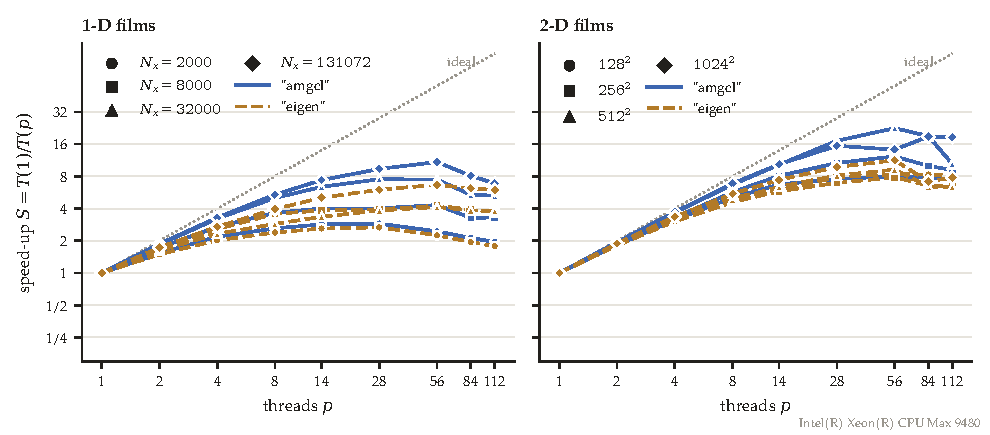
\includegraphics[width=\textwidth]{figures/parallel-scaling.pdf}
  \caption{The speed-up of \cref{tab:scaling} against the thread count, every
    size and both backends, with the ideal $S = p$ dotted. Both backends scale
    on the large films, \val{"amgcl"} further; the small 1-D film stops
    near $3\times$, and almost every case falls off past one socket (56
    threads). Drawn by \file{docs/manual/\bk figures/\bk make\_scaling.py} from
    \file{tools/scaling/\bk results/\bk scaling-mc076.tsv}.\label{fig:parallel-scaling}}
\end{figure}

\Cref{fig:parallel-scaling} shows the same numbers as curves. Four readings.

\paragraph{Both backends scale, \val{"amgcl"} further.}
At 56 threads \val{"eigen"} reaches $8\times$ to $11\times$ in 2-D and
\val{"amgcl"} $8\times$ to $22\times$, the larger factors on the larger films.
\val{"eigen"}'s preconditioner is a block-Jacobi ILUT whose blocks are
factorized in parallel (\cref{sec:linsolve:eigen}); what limits it is the
BiCGStab iterations, 33 to \SI{72}{\percent} of the loop, whose vector work is
sequential (\cref{sec:parallel:profile}). AMGCL threads its set-up and its
iterations alike.

\paragraph{Which backend is faster depends on the thread count.}
In 1-D the two are level at $N_x = 2000$, where AMGCL solves the system
directly (within \SI{9}{\percent} on one thread and \SI{2}{\percent} at 28),
and \val{"eigen"} is ahead at every thread count from $8000$ to $32000$:
$5.8\times$ on one thread and $5.7\times$ at 56 at $N_x = 8000$. AMGCL has
little to coarsen on a one-dimensional problem and needs about 100 linear
iterations a solve there, where Eigen needs 12. At $N_x = 131072$ the two are
within \SI{11}{\percent} on one thread and \val{"amgcl"} is $1.5\times$ faster at 56. In 2-D the
two are level at $128^2$; from $256^2$ up \val{"eigen"} is faster on one
thread ($1.4\times$ at $256^2$, $1.6\times$ at $512^2$, $1.2\times$ at
$1024^2$) and on eight threads up to $512^2$, and \val{"amgcl"} from 8 to 28
threads up ($1.1\times$ at 56 on $256^2$, $1.5\times$ on $512^2$,
$1.4\times$ at 28 on $1024^2$). \Cref{sec:parallel:backend} turns this into a
rule.

\paragraph{The useful thread count is 28--56, not 112.}
Every case but one is at or past its optimum by 56 threads and slower at 112
than at 56. The two sockets carry 8 NUMA nodes, and past one
socket the reductions and the memory traffic cost more than the extra cores
return; this is why a run uses at most one socket (\cref{sec:parallel:cap}).
The exception, \val{"amgcl"} on $1024^2$, is fastest at 84 threads, in
\SI{18}{\percent} less time than at 28; at 56 its three repeats spread by
\SI{22}{\percent}. (The \val{"amgcl"} row of $N_x = 2000$ was measured
again on another node of the same kind, after a fix to AMGCL's coarsest level;
\val{"eigen"} timed there agreed with \cref{tab:scaling} to \SI{2}{\percent}.)

\paragraph{Small problems do not parallelize.}
At $N_x = 2000$ the best speed-up is $2.7\times$ with \val{"eigen"} and
$2.9\times$ with \val{"amgcl"}, both at 28 threads, and past that more threads
cost time. Below a few thousand points,
run one thread per case and put several cases side by side. The kit that
measured \cref{tab:scaling} turns the thread limit off, so that every row is
the thread count asked for.

\begin{note}[Reading the Amdahl fit in the summary tool]
  \file{tools/scaling/summarize.py} prints a fitted parallel fraction $f$.
  Where a case slows down past its optimum the fit reports $f = 0.000$, which
  does not mean nothing is parallel: Amdahl's law can express saturation but
  not slowdown, so the regression has nothing to fit. Read $S$ and $E$,
  which are measured, in preference to $f$, which is a model.
\end{note}

\section{Which backend to ask for}
\label{sec:parallel:backend}

The measurements above give the following rule. The penalty for getting it
wrong is large only in 1-D; in 2-D the two backends are within a factor of
1.6 of each other at every size up to one socket of threads.

\begin{yzntable}{Backend by problem shape\label{tab:backend-rule}}{@{}L{0.22\textwidth} L{0.16\textwidth} L{0.50\textwidth}@{}}
\textsf{\bfseries Problem} & \textsf{\bfseries Backend} & \textsf{\bfseries Why}\\ \midrule
1-D, up to $\sim 10^4$--$10^5$ cells & \val{"eigen"} & AMGCL has almost nothing to coarsen and spends eight times the linear iterations: $5.7\times$ slower at $N_x=8000$. Level at $N_x = 2000$, where AMGCL solves directly. \\
1-D, $\sim 10^5$ cells and more & either & Within \SI{11}{\percent} on one thread; \val{"amgcl"} $1.5\times$ faster at 56 threads on $N_x = 131072$. \\
2-D, a socket of threads & \val{"amgcl"} & $1.1$--$1.5\times$ faster from $256^2$ up, level at $128^2$. \\
2-D, eight threads or fewer & \val{"eigen"} & Faster from $256^2$ up on one thread, by $1.2$--$1.6\times$. \\
\end{yzntable}

\val{"auto"} asks the film's in-plane dimension and returns \val{"eigen"} for
a 1-D film and \val{"amgcl"} for a 2-D one. The default is \val{"auto"}, so
leaving the key alone gives the faster backend in 1-D below $\sim 10^5$
cells and on a full socket in 2-D. On a small machine and a 2-D film of
$256^2$ or more, set \key{Backend} to \val{"eigen"}.

\begin{note}[Why there is no size or thread threshold]
  Where one backend overtakes the other depends on the machine, and outside
  1-D the gain is small either way. A threshold would put a machine-dependent
  guess into the solver, so \val{"auto"} splits on the dimension alone. If the
  run time of a long study matters, measure both on your machine
  (\cref{sec:parallel:kit}) and set \key{Backend} explicitly.
\end{note}

\section{Measuring it on your own machine}
\label{sec:parallel:kit}

\file{tools/scaling/} is a self-contained kit for exactly this measurement:
generated cases, a sweep script, and a summarizer.

\begin{shell}
cmake -S . -B build -DCMAKE_BUILD_TYPE=Release -DYUZEN_WITH_AMGCL=ON
cmake --build build -j

tools/scaling/scaling.sh --tier quick --repeats 1 --threads "1 4"
tools/scaling/scaling.sh --threads "1 2 4 8 16 32 64" --repeats 3
python3 tools/scaling/summarize.py tools/scaling/results/scaling-*.tsv
\end{shell}

The sweep appends one row per run to a tab-separated file that carries the
machine's identity in its header, and it skips rows it already has, so an
interrupted sweep is restarted by repeating the command. What makes the
numbers comparable is that the cases fix the work: the time step is constant
(\key{Numerics.TimeStepControl} disabled), the step count is fixed
(\key{Numerics.MaxSteps}), and field output is off --- the output interval
also caps the time step, so leaving it on would change the work per step as
well as the time spent writing. What is timed is the time-step loop alone,
taken from \file{JobInfo.txt}, not the whole process, so grid construction and
start-up do not dilute the result.

\begin{warn}[Small cases cannot use a large machine, whatever you do]
  The reductions in \code{Vector} are split into a fixed number of blocks,
  $\min(256,\,N/512)$ for $N$ elements, so that the answer does not depend on
  the thread count (\cref{sec:repro:reduction}). Two limits follow. A case
  with fewer than $512p$ unknowns cannot give all $p$ threads a block at all
  --- at 112 threads that is 57\,344 unknowns, and a comfortable margin needs
  131\,072 so that the block count reaches its ceiling. And because the
  ceiling is 256 blocks, \textbf{beyond 256 threads the reductions do not
  parallelize any further}. That ceiling is the price of bit-identity, and it
  is deliberate.

  This is why the kit's ladder goes up to $1024^{2}$ in 2-D and $N_x =
  131\,072$ in 1-D. The small cases are in it to show the other end: that they
  do not speed up, and should be run one thread each, several at a time.
\end{warn}

\subsection{Where the time goes}
\label{sec:parallel:profile}

With \env{YUZEN\_PROFILE=1} the solver times named parts of the run and
writes the totals to standard error at exit, one line each (name, calls,
seconds):
\begin{shell}
[profile] threads 8
[profile] h.linsolve        2030      0.097730
\end{shell}
\begin{yzntable}{The parts \env{YUZEN\_PROFILE} times. Times of nested parts are each inclusive: \code{h.linsolve} contains the \code{lin.*} of the film height.\label{tab:profile-parts}}{@{}L{0.20\textwidth} L{0.72\textwidth}@{}}
\textsf{\bfseries Name} & \textsf{\bfseries What}\\ \midrule
\code{step}        & one time step, all of it \\
\code{output}      & the field and history output between steps \\
\code{h.assemble}  & the film-height matrix (\code{SetMatrixA}) \\
\code{h.jacobian}  & its Jacobian and the matrix of the implicit step \\
\code{h.rhs}       & the explicit part and the right-hand side \\
\code{h.linsolve}  & the linear solve of the film height \\
\code{h.couple}    & the rest of a Newton pass, the well-mixed concentration trial among it \\
\code{h.after}     & the end of the step, the concentration of the step among it \\
\code{c.solve}     & a concentration solve, all of it; \code{c.linsolve} its linear solve \\
\code{velocity}    & the velocities \\
\code{lin.prepare} & handing the matrix to the backend: gathering, scaling, copying \\
\code{lin.precond} & building the preconditioner (ILUT factorization, AMG set-up) \\
\code{lin.iterate} & the BiCGStab iterations \\
\end{yzntable}
A scope inside a parallel region times nothing; what is timed is what the
thread running the time loop sees. \file{tools/profile\_threads.py} runs a
set of cases with both backends at each thread count, with the cap of
\cref{sec:parallel:cap} off, and tabulates the parts against the thread count;
it measures in pieces under a batch time limit as
\file{tools/case\_runtimes.py} does (\cref{sec:env:tools}).

On a Xeon Max 9480 node like that of \cref{tab:scaling} it shows where the limits of
\cref{sec:parallel:scaling} come from. With \val{"eigen"} on the 2-D films of
\cref{tab:scaling}, building the block-Jacobi ILUT preconditioner takes 6--30\,\%
of the time-step loop, the larger shares on the smaller grids, and the BiCGStab
iterations 33--72\,\%, the larger shares on the larger grids; on the $60\times60$
film of \file{leveling\_2d\_reg} the factorization takes 55--61\,\%, because its
blocks stop dividing the work at four threads. With \val{"amgcl"}, the AMG set-up
is rebuilt at every linear solve, five to eight times a step (about three
for the film height, two to four for the concentration), and it scales less well than the
iterations: its share of the loop grows from 4--9\,\% on one
thread to 10--28\,\% at 56, the larger
shares on the smaller grids. Handing the matrix to the backend takes
0--3\,\% on the 2-D cases at every thread count.

\section{Speed and reproducibility are separate questions}
\label{sec:parallel:repro}

Changing the thread count does not change the answer. With \val{"eigen"} the
result is bit-identical, and the test suite asserts it
(\cref{ch:reproducibility}); with \val{"amgcl"} it moves in the last few digits
(\cref{sec:verification:amgclthreads}). So the choice of thread count is purely
a performance decision, and the choice of backend is the one that has a
correctness dimension to it. If you need bit-identical results across machines
as well as across thread counts, fix the backend to \val{"eigen"} and accept
the slower 2-D solve.
